%%%%%%%%%%%%%%%%%%%%%%%%%%%%%%%%%%%%%%%%%
% a0poster Portrait Poster
% LaTeX Template
% Version 1.0 (22/06/13)
%
% The a0poster class was created by:
% Gerlinde Kettl and Matthias Weiser (tex@kettl.de)
% 
% This template has been downloaded from:
% http://www.LaTeXTemplates.com
%
% License:
% CC BY-NC-SA 3.0 (http://creativecommons.org/licenses/by-nc-sa/3.0/)
%
%%%%%%%%%%%%%%%%%%%%%%%%%%%%%%%%%%%%%%%%%

%----------------------------------------------------------------------------------------
%	PACKAGES AND OTHER DOCUMENT CONFIGURATIONS
%----------------------------------------------------------------------------------------

\documentclass[a0,portrait]{a0poster}

\usepackage[utf8]{inputenc} %para aceitar carcteres da língua portuguesa
\usepackage[brazil]{babel}
\setlength\parindent{30pt}

\usepackage{multicol} % This is so we can have multiple columns of text side-by-side
\columnsep=100pt % This is the amount of white space between the columns in the poster
\columnseprule=3pt % This is the thickness of the black line between the columns in the poster

\usepackage[svgnames]{xcolor} % Specify colors by their 'svgnames', for a full list of all colors available see here: http://www.latextemplates.com/svgnames-colors

\usepackage{times} % Use the times font
%\usepackage{palatino} % Uncomment to use the Palatino font

\usepackage{graphicx} % Required for including images
%\graphicspath{{figures/}} % Location of the graphics files
\usepackage{booktabs} % Top and bottom rules for table
\usepackage[font=small,labelfont=bf]{caption} % Required for specifying captions to tables and figures
\usepackage{amsfonts, amsmath, amsthm, amssymb} % For math fonts, symbols and environments
%\usepackage{wrapfig} % Allows wrapping text around tables and figures

\begin{document}

%----------------------------------------------------------------------------------------
%	POSTER HEADER 
%----------------------------------------------------------------------------------------

% The header is divided into two boxes:
% The first is 75% wide and houses the title, subtitle, names, university/organization and contact information
% The second is 25% wide and houses a logo for your university/organization or a photo of you
% The widths of these boxes can be easily edited to accommodate your content as you see fit

\begin{minipage}[b]{0.75\linewidth}
{\centering
%\veryHuge \color{NavyBlue} \textbf{Projeto e Controle  de Processo com Controle de Nível, Vazão e Temperatura} \color{Black}\\[2cm] % Title
\fontsize{90}{120} \color{NavyBlue} \textbf{Projeto e Controle  de Processo com Controle de Nível, Vazão e Temperatura} \color{Black}\\[1.5cm] % Title

%\Huge\textit{An Exploration of Complexity}\\[2cm] % Subtitle
\huge \textsc{Luan R. P. Medeiros e Eduardo S. Tognetti}\\[0.5cm] % Author(s)

\Large{\bf Departamento de Engenharia Elétrica, ENE/FT/UnB, Brasília, DF, Brasil}\\[0.5cm]
\Large Emails: \texttt{luan.rafael@hotmail.com e estognetti@ene.unb.br}\\
}
\end{minipage}
%
\begin{minipage}[b]{0.25\linewidth}

\includegraphics[width=10cm]{logo.png}\\
\end{minipage}

\vspace{2cm} % A bit of extra whitespace between the header and poster content

%----------------------------------------------------------------------------------------

\begin{multicols}{2} % This is how many columns your poster will be broken into, a portrait poster is generally split into 2 columns

%----------------------------------------------------------------------------------------
%	RESUMO
%----------------------------------------------------------------------------------------

\color{NavyBlue} % Navy color for the abstract
\begin{abstract}

\fontsize{18}{22}
Este projeto aborda o problema de controle de nível e temperatura de um processo didático envolvendo mistura de soluções. Deseja-se controlar a temperatura e o nível de água em um tanque com o uso de controladores PI e PID, e estratégias de controle tipicamente empregadas em plantas industriais. São apresentadas três estratégias de controle: uma monovariável e duas multimalhas.

\end{abstract}
\vspace{0.5cm}
%----------------------------------------------------------------------------------------
%	INTRODUÇÃO
%----------------------------------------------------------------------------------------
%\fontsize{45}{55}

\color{DarkSlateGray} % SaddleBrown color for the introduction

\section*{Introdução}

\color{Black}

Processos com controle temperatura e nível são usuais nas indústrias de alimentos e químicas, e geralmente demandam altos valores energéticos. São apresentadas diferentes estratégias para o controle de temperatura e nível de um processo possível de ser implementado para fins didáticos. 
%----------------------------------------------------------------------------------------
%	DESCRIÇÃO DO SISTEMA
%----------------------------------------------------------------------------------------
\vspace{1cm}
\color{DarkSlateGray} % DarkSlateGray color for the rest of the content

\section*{Descrição do Sistema}

\color{Black}

O processo é composto por dois tanques ligados pela base, e o fluxo de água provém de duas bombas. \\
\indent A representação do processo é a seguinte:

\begin{center}\vspace{1.5cm}
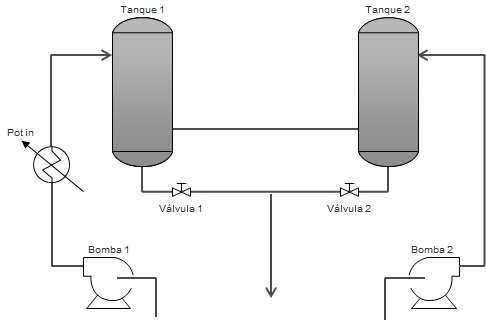
\includegraphics[width=0.78\linewidth]{descricao}
\captionof{figure}{Processo de mistura.}
\end{center}\vspace{1.5cm}

Descrição: a água proveniente da bomba 1 passa pelo estágio de aquecimento e entra no tanque 1. 
O tanque 2 é alimentado com água em temperatura ambiente através da bomba 2, e também com água aquecida do tanque 1 por meio de uma tubulação de ligação. 



%----------------------------------------------------------------------------------------
%	MODELAGEM MATEMÁTICA
%----------------------------------------------------------------------------------------
\vspace{1cm}
\color{DarkSlateGray} % SaddleBrown color for the introduction

\subsection*{Modelagem Matemática}

\color{Black}

O Teorema de Torricelli foi aplicado para determinar a velocidade de saída média dos tanques $V_r$. Com isso, determinam-se fluxos de saída do tanque 2 e o do tanque 1 ao tanque 2, em que foi considerado o nível relativo dos tanques:

\vspace{0.2cm}
\begin{equation}
F_{out} = \pi \cdot r_{out}^{2} \cdot V_r
\end{equation}
\vspace{0.4cm}

Aplicou-se o princípio de consevação de massa para obter a dinâmica do nível dos tanques:

\vspace{0.2cm}
\begin{equation}
\frac{dH}{dt} =  \frac{\sum F_{in} - \sum F_{out}}{A_{transversal}}
\end{equation}
\vspace{0.4cm}


Para descrição da dinâmica da temperatura nos tanques aplicou-se o balanço de energia para cada elemento do sistema: unidade de aquecimento, tanque 1 e tanque 2:

\vspace{0.2cm}
\begin{equation}
\frac{dT}{dt} =  \frac{\sum{F_{in} \cdot T_{in}} - \sum{F_{out} \cdot T}}{Volume} + \frac{Pot \cdot cp \cdot \rho}{Volume}
\end{equation}
\vspace{0.2cm}


%----------------------------------------------------------------------------------------
%	LINEARIZAÇÃO E FUNÇÕES DE TRANSFERÊNCIA
%----------------------------------------------------------------------------------------

\color{DarkSlateGray} % SaddleBrown color for the introduction

\subsection*{Linearização e Funções de Transferência}

\color{Black}

A linearização valeu-se do uso de variáveis de desvio. Define-se um ponto de operação do sistema, com níveis e temperaturas fixas. As funções de transferência do sistema são determinadas para este ponto, garantindo condições iniciais nulas. 
% eqs. 6 a 8


%----------------------------------------------------------------------------------------
%	ESTRATÉGIAS DE CONTROLE E SINTONIA
%----------------------------------------------------------------------------------------
\vspace{1cm}
\color{DarkSlateGray} % SaddleBrown color for the introduction

\section*{Estratégias de Controle e Sintonia}

\color{Black}

Com base nos modelos matemáticos e no comportamento do sistema, foram definidas as estratégias de controle simples, cascata e cruzado. A sintonia dos controladores PI e PID é baseada no método IMC (do inglês Internal Model Controller) de Skogestad. Os controladores foram sintonizados a partir das funções de transferência, e as simulações foram realizadas com a representação não linear do processo. 

\begin{center}\vspace{5cm}
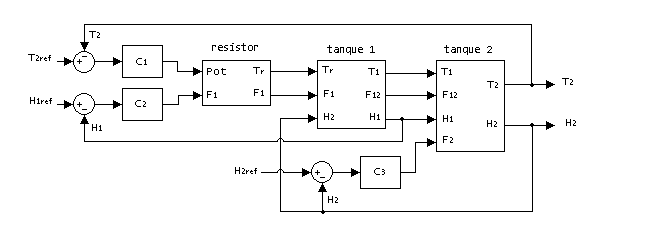
\includegraphics[width=0.75\linewidth]{simples}
\captionof{figure}{Simples.}
\end{center}

\begin{center}\vspace{0.5cm}
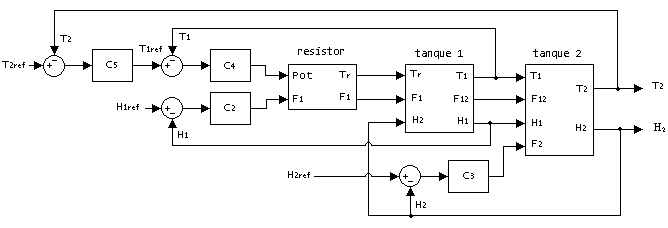
\includegraphics[width=0.75\linewidth]{cascata}
\captionof{figure}{Cascata.}
\end{center}

\begin{center}
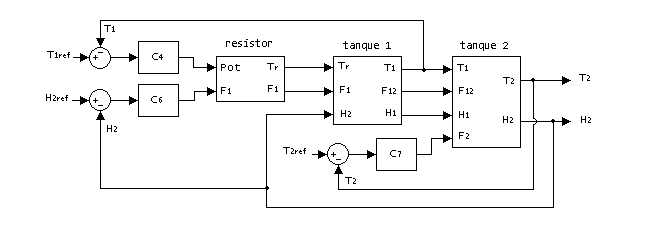
\includegraphics[width=0.75\linewidth]{cruzado}
\captionof{figure}{Cruzado.}
\end{center}



%----------------------------------------------------------------------------------------
%	ANÁLISE DOS RESULTADOS 
%----------------------------------------------------------------------------------------

\color{DarkSlateGray} % SaddleBrown color for the introduction

\section*{Análise dos Resultados}

\color{Black}

Simulou-se estratégias de controle em malha fechada. Sinais do tipo degrau foram usados para referências de $H_2$ e $T_2$.\\
\indent O resultado da simulação das estratégias de controle em malha fechada é mostrado abaixo:

\vspace{0.8cm}
\begin{minipage}{.5\linewidth}
    \begin{center}
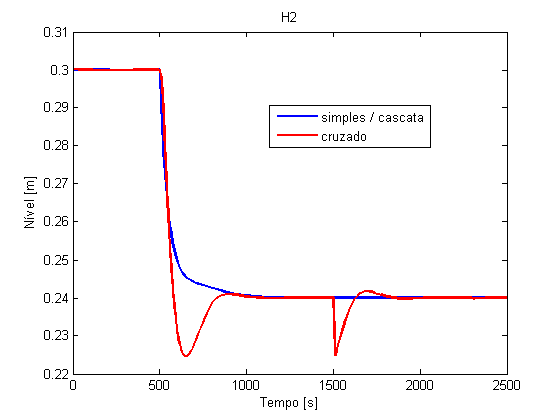
\includegraphics[width=1\linewidth]{H2_color}
\captionof{figure}{Nível do tanque 2.}
\end{center}
  \end{minipage}%
  \begin{minipage}{.5\linewidth}
    \begin{center}
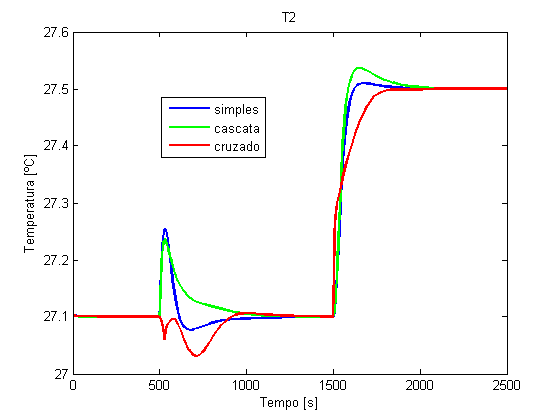
\includegraphics[width=1\linewidth]{T2_color}
\captionof{figure}{Temperatura do tanque 2.}
\end{center}
  \end{minipage}
\vspace{0.5cm}


São usados indicadores de desempenho nas variáveis $H_2$ e $T_2$: a integral do erro absoluto (IAE), a integral do quadrado do erro (ISE), distúrbio (Dist), valor de pico do erro causado por distúrbio, e sobresinal (M).

\begin{center}\vspace{1cm}
\begin{tabular}{l l l l l}
\toprule
\textbf{Estratégia \hspace{0.5cm}} & \textbf{IAE \hspace{0.8cm} } & \textbf{ISE \hspace{0.8cm}} & \textbf{Dist (cm) \hspace{0.4cm}} & \textbf{M (cm) } \\
\midrule
Simples & 3.91 & 0.09 & 0 & 0 \\
Cascata & 3.91 & 0.09 & 0 & 0 \\
Cruzado & 5.81 & 0.14 & 1.51 & 1.54 \\
\bottomrule
\end{tabular}
\captionof{table}{Indicadores quantitativos de $H_2$ para um degrau de 6 cm.}
\end{center}\vspace{1cm} 

\begin{center}
\begin{tabular}{l l l l l}
\toprule
\textbf{Estratégia \hspace{0.5cm}} & \textbf{IAE \hspace{0.8cm} } & \textbf{ISE \hspace{0.8cm}} & \textbf{Dist ($º$C) \hspace{0.4cm}} & \textbf{M ($º$C) } \\
\midrule
Simples & 34.45 & 6.24 & 0.153 & 0.010 \\
Cascata & 43.46 & 6.29 & 0.136 & 0.037  \\
Cruzado & 40.42 & 4.48 & 0.068 & 0  \\
\bottomrule
\end{tabular}
\captionof{table}{Indicadores quantitativos de $T_2$ para um degrau de 0.4 $º$C.}
\end{center}\vspace{1cm} 


É observado que nas estratégias simples e cascata o controle de nível é melhor, pois a malha de temperatura está desacoplada. Com a estratégia cascata é possível atenuar um distúrbio na temperatura do tanque 1 antes que atinja o tanque 2. Na estratégia cruzado o controle de temperatura afeta o controle de nível.


%----------------------------------------------------------------------------------------
%	CONCLUSÃO
%----------------------------------------------------------------------------------------
\color{DarkSlateGray} % SaddleBrown color for the introduction

\section*{Conclusão}

\color{Black}

Foi descrito o processo de controle de nível e temperatura de tanques. O sistema foi modelado, linearizado em torno do ponto de operação e sua representação em funções de transferência foi obtida. Utilizou-se controladores PI e PID, sintonizados pelas funções de transferência. Três estratégias de controle foram implementadas computacionalmente e comparadas. Estratégias de controle mais avançadas podem ser aplicadas para este sistema futuramente. 


%----------------------------------------------------------------------------------------

\end{multicols}
\end{document}
